\subsection{Copy Optimization}
Copy optimizations involve copying and rearranging some or all of a piece of
data into a chunk of memory such that operating on the copied data is more
efficient than operating on the original data.

In the context of a naive matrix multiplication $A \times B$, the innermost
loop of the multiplication accesses matrix $B$ with unit stride but accesses
matrix A with a stride of $M$ where $M$ is the number of rows and columns of
$A$ and $B$. This non-unit stride vastly reduced how effectively we could
operate on matrix $A$. First, the large stride has poor spatial locality which
can lead to poor caching. Similarly, operating on non-contiguous elements of
$A$ makes vectorization hard or impossible.

To solve this problem, we used a copy optimization in which we simply
transposed $A$ to a new array in row-major order. This allowed us to access
both $A$ and $B$ in unit stride in the innermost loop.

Our use of copy optimizations was the most successful approach that we found
for increasing performance. This alone boosted our performance above all other
implementations except for MKL and OpenBLAS, as shown in \figref{copy}.

\begin{figure}[h]
  \centering
  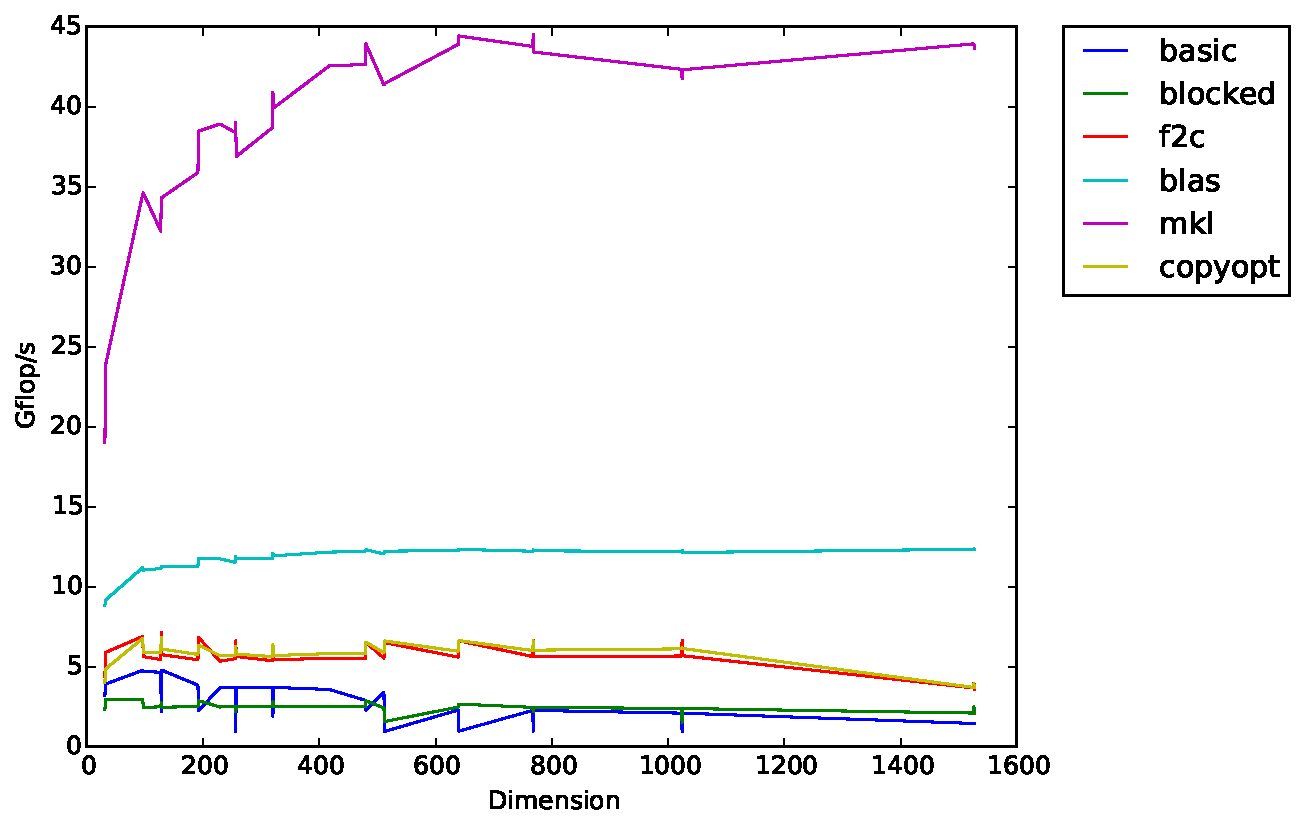
\includegraphics[width=\textwidth]{img/timing_copyopt.pdf}
  \caption{Performance of matrix multiplication with copy optimization.}
  \label{fig:copy}
\end{figure}
